\section{Reductions II}
\begin{itemize}
	\item Recap: Two computational problems \(A\) and \(B\), and \(A\) reduces (in polynomial time) to \(B\) 
		is written as \(A \preceq_p B\). This means that if an algorithm exists to solve \(B\) in polynomial 
		time, then that same algorithm can be used to solve \(A \) in polynomial time. 

		\question{Is this restricted to only polynomial time? Shouldn't any feasible algorithm that solves 
		\(B\) also solve \(A\)?}
		
		\question{Why are we so concerned about polynomial time? Do similar problems exist if we define 
		``efficient'' to be exponential time?}
	\item Also recall the diagram we made to represent this process of reducing \(A\) to \(B\), via 
		a polynomial time reduction and recovery algorithm. Note that these two algorithms \textbf{must} execute
		in polynomial time. 
		\begin{itemize}
			\item We can prove that \(A \preceq_p B\) even if \(A, B\) are not known to be efficient.
		\end{itemize}
	\item We also saw two reductions: zero sum games reducing to LP, and Hamiltonian cycle reducing to min-TSP.
	\item Transitivity: If \(A \preceq_p B \preceq_p C\), then \(A \preceq_p C\). 
\end{itemize}
\subsection{Common mistakes in Reductions}
\begin{itemize}
	\item If we're asked to prove that \(A \preceq_p B\), we need to come up with an algorithm that takes
		\(A\) to \(B\), not \(B\) to \(A\). Make sure you check that you're proving the correct direction!
\end{itemize}
\subsection{Landscape of Problems}
\begin{itemize}
	\item We're going to use the below diagram to show the problems:
		\begin{center}
			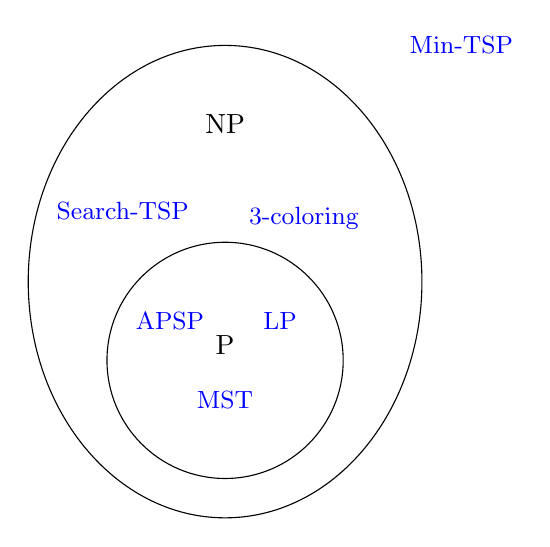
\begin{tikzpicture}
				\draw(0, 0) circle [radius=1.5cm];
				\draw node at (0, 0.2) {P};
				\draw (0, 1) ellipse [x radius = 2.5, y radius = 3];
				\draw node at (0, 3) {NP};
				\draw[blue] node at (0, -0.5) {\small MST};
				\draw[blue] node at (0.7, 0.5) {\small LP};
				\draw[blue] node at (-0.7, 0.5) {\small APSP};
				\draw[blue] node at (1, 1.8) {\small 3-coloring}; 
				\draw[blue] node at (-1.3, 1.9) {\small Search-TSP};
				\draw[blue] node at (3, 4) {\small Min-TSP};
			\end{tikzpicture}
		\end{center}
	\item We're not going to prove this, but it has been shown that factoring reduces to the 3-coloring 
		problem. Similarly, factoring also reduces to the Rudrata Cycle problem. 
	\item It turns out that every problem in NP reduces to Rudrata cycle!
	\item These are the most difficult problems in NP, and it can be shown that every problem in NP reduces 
		to an NP-complete problem
	\item \textbf{NP-Hardness:} A problem \(A\) is NP-hard if every problem \(B\) in NP reduces to \(A\). 
	\item \textbf{NP-Completeness:} A problelm \(A\) is NP-complete if \(A \in \text{NP}\) and \(A\) is 
		NP-hard.
	\item Problems in NP that aren't NP-complete are called an \textbf{NP-intermediate} problem 
	\item \textbf{Fact:} Given two problems that are NP-complete, then \(A \preceq_p B\) and \(B \preceq_p A\). 
		So this means that you can basically think of \(A\) and \(B\) are basically equivalent problems. 

		\question{Is this a biconditional?}

		\answer{No, consider two problems in P: they can be reduced to one another, but they are not 
		in NP.} 
		\begin{itemize}
			\item  There are thousands upon thousands of NP-complete problems, and by notion of reduction, 
				they are (in some sense) the same problem.
			\item This also means that if there exists a polynomial time algorithm for any NP-problem, 
				then this would imply that P = NP.
		\end{itemize}
		\question{How is it that if P = NP then every problem becomes NP-complete?}  
\end{itemize}

\subsection{Proving NP-Completeness}
\begin{itemize}
	\item Cook-Levin Theorem: showed that every problem in NP reduces in polynomial time to a circuit SAT 
		problem.
	\item It can then be shown that circuit-SAT reduces to 3-SAT, making 3-SAT an NP-complete problem. In 
		terms of a diagram:
		\begin{center}
			\begin{tikzpicture}[every text node part/.style={align=center}]
				\foreach \x in {0, 4}
						\draw[-stealth] (\x+0.5, 0) -- (\x+2, 0);
				\draw node at (-1, 0) {Every problem \\ in NP};
				\draw node at (3.25, 0) {Circuit\\SAT};
				\draw node at (7.25, 0) {3-SAT};
				\draw [-stealth] (8, 0) -- (10, 1.5) node[right] {Independent \\ Set};
				\draw [-stealth] (8, -0.2) -- (10, -1.5) node[right] {Rudrata Cycle};
			\end{tikzpicture}
		\end{center}
		\question{Finish this Diagram Later}
	\item To show that a problem is NP-complete, we first show that \(A \in \text{NP}\), then 
		pick some problem \(B\) that is known to be NP-complete and show that \(B \preceq_p A\). 
		
		\question{What if we show that \(A \preceq_p B\)?}

		\answer{We don't need to, since \(A \preceq_p B\) is true already because \(B\) 
		is an NP-complete problem!}
\end{itemize}
\subsection{Circuit SAT}
\begin{itemize}
	\item A Boolean circuit is a directed acyclic graph with:
		\begin{itemize}
			\item Input nodes \(x_1, \dots, x_n\) 
			\item one output node, with an output \(C(x)\)
			\item gates marked OR, AND, NOT: \(\lor, \land, \neg\)
		\end{itemize}
		A possible graph is:
		\begin{center}
			\begin{tikzpicture}
				\node (c) {$\lor$}
					child [stealth-] {node (a) [left] {$\land$}  
					child {node {$x_1 = 1$}}
				}
				child [stealth-] {node {$\land$}
				  child {node (b) {\(x_2 = 1\)} }
				  child {node {\(\neg\)} 
					  child {node {\(x_3 = 1\) }}
					}
				};
			\draw[-stealth] (b) -- (a);
			\draw[-stealth] (c) -- (0, 1) node[above]  {1}; 
			\end{tikzpicture}
		\end{center}	
	\item The input to circuit SAT is a circuit \(C\) with \(n\) inputs and \(m\) referring to the number of 
		gates. We want to output an assignment of \((x_1, \dots x_n)\) such that \(x_i \in \{0, 1\}\) 
		such that \(C(x) = 1\).
	\item By the Cook-Levin theorem, circuit-SAT is NP-complete. As for a bit of intuition on why this is true, 
		you can think of every problem as basically a collection of logical inputs, which basically means 
		that every problem can be reduced to some complex circuit of logical gates.  
\end{itemize}
\subsubsection{3-SAT}
\begin{itemize}
	\item Here, we're given \(n\) Boolean variables \( x_1, \dots, x_n\) such that \(x_i \in \{0, 1\} \), and 
		\(m \le  3\) variable clauses that join the variables together. 
	\item We want to output an assignment of \(x_1, \dots, x_n\) that satisfies all the clauses. 
	\item \textbf{Theorem:} Circuit-SAT reduces to 3-SAT

		\textit{Proof:} Suppose we're given an input to a circuit-SAT problem.
\end{itemize}
